% !TEX TS-program = pdflatex
\documentclass{article}
\usepackage[margin=1in]{geometry}

% --- packages
\usepackage{amsmath,amssymb}
\usepackage{xcolor}
\usepackage{hyperref}
\hypersetup{
  colorlinks=true,
  linkcolor=blue!70!black,
  urlcolor=cyan!70!black,
  citecolor=green!50!black
}
\usepackage{tikz}
\usetikzlibrary{calc}

% --- macros
\newcommand{\dist}[2]{\lVert #1-#2\rVert}

% --- meta
\title{Limitations of the Monotonic Relative Neighborhood Graph for External Query Points}
\author{}
\date{\today}

\begin{document}
\maketitle

\section{Introduction}
The \emph{Monotonic Relative Neighborhood Graph} (MRNG) is a sparse proximity graph introduced by Fu\,\textit{et\,al.}\,\cite{fu2017nsg} as an ideal backbone for graph\hyp based approximate nearest\hyp neighbour (ANN) search. An MRNG guarantees that from every vertex $u$ there exists a strictly distance\hyp decreasing path to any other vertex $v$\,---a property often called \emph{monotone navigability}. Recent work by Zhu and Zhang\,\cite{zhu2021mrng} gives a theoretical account of why such graphs achieve near\hyp logarithmic greedy search time.

In practice, however, ANN systems must answer queries that are \emph{not} present in the original data set. This note gives a simple planar counter\hyp example showing that the MRNG's monotone property does \emph{not} extend to external query points: a greedy walk can get trapped in a local minimum even when the true nearest neighbour is one hop away.

Figure~\ref{fig:mrng-diagram} visualises the construction and the failing search path.

\section{MRNG Construction Recap}
Given a finite set $P\subset\mathbb R^{d}$, the MRNG is defined as follows\,\cite{fu2017nsg}:
\begin{itemize}
  \item \textbf{Vertices.} Each data point in $P$.
  \item For every ordered pair $(u,v)$, let $L(u,v)=\{x\mid \dist{x}{u}<\dist{u}{v}\ \wedge\ \dist{x}{v}<\dist{u}{v}\}$ be the \emph{lune}.
  \item \textbf{Edge rule.} Sort $P\setminus\{u\}$ by distance to $u$. Insert a directed edge $u\rightarrow v$ iff $L(u,v)$ contains no point $w$ that already has an outgoing edge from $u$.
\end{itemize}
The resulting graph has constant average degree, is strongly connected, and supports distance\hyp decreasing greedy walks between any two data points.

\section{Failure for External Queries}
Suppose a query point $q\notin P$ is introduced (Figure~\ref{fig:mrng-diagram}). Starting the greedy walk at $p_1$ yields the path $p_1\rightarrow p_2\rightarrow p_3$, where the walk terminates because no neighbour of $p_3$ is closer to $q$ than $p_3$. Yet the true nearest neighbour is $p_5$. Thus the MRNG guarantee does not suffice for ANN systems that must serve arbitrary queries.

\paragraph{Implication.} Production systems therefore approximate MRNG with super\hyp graphs such as NSG\,\cite{fu2017nsg} or add multi\hyp entry\hyp point and backtracking heuristics\,\cite{zhu2021mrng}.

\section{Conclusion}
\begin{itemize}
  \item The MRNG ensures monotone connectivity for \emph{in\hyp graph} searches.
  \item External queries can defeat a pure greedy walk.
  \item Practitioners should augment the graph (NSG, HNSW) or the search procedure (multi\hyp entry, beam search) to restore recall.
\end{itemize}

\begin{figure}[t]
  \centering
  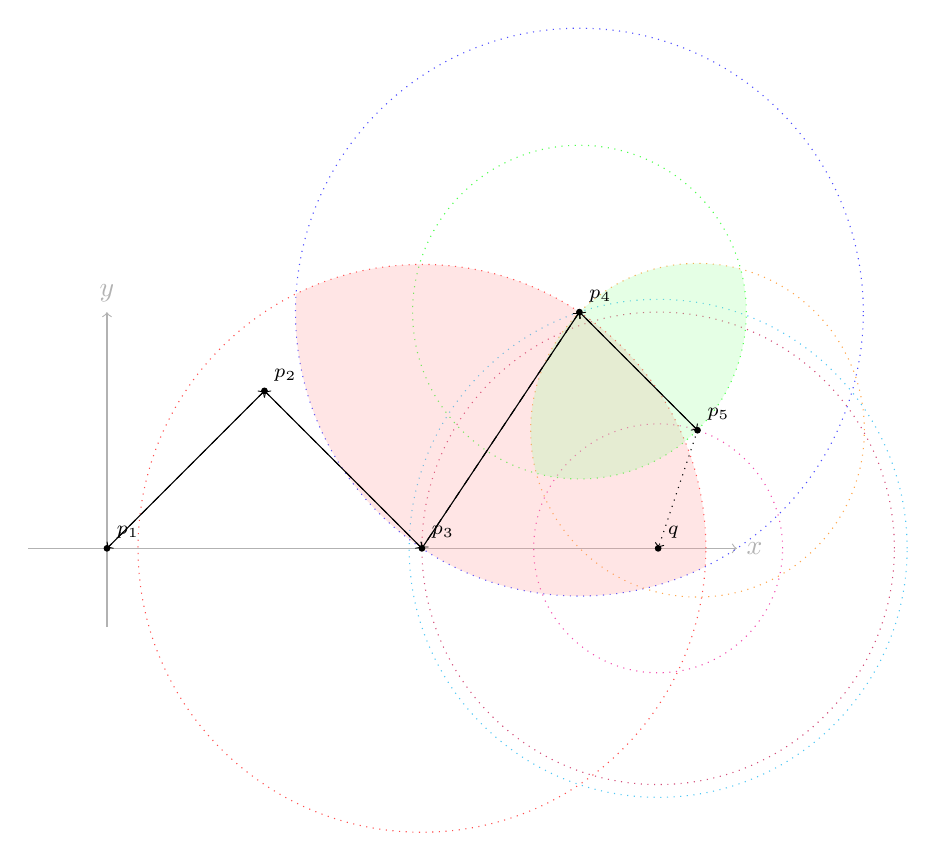
\begin{tikzpicture}[scale=0.5]
    % --- coordinates
    \coordinate (p1) at (0,0);
    \coordinate (p2) at (4,4);
    \coordinate (p3) at (8,0);
    \coordinate (p4) at (12,6);
    \coordinate (p5) at (15,3);
    \coordinate (q)  at (14,0);

    % --- axes (subtle)
    \draw[->,gray!60] (-2,0) -- (16,0) node[right]{$x$};
    \draw[->,gray!60] (0,-2) -- (0,6)  node[above]{$y$};

    % --- helper macro to draw circles lightly
    \def\lcircle[#1]#2#3{\draw[#1,dotted,thin] let \p1=(#2), \p2=(#3), \n1={veclen(\x2-\x1,\y2-\y1)} in (#2) circle (\n1);}

    % --- circles
    \lcircle[red!70]  {p3}{p4}
    \lcircle[blue!70] {p4}{p3}
    \lcircle[green!70]{p4}{p5}
    \lcircle[orange!70]{p5}{p4}
    \lcircle[purple!70]{q}{p3}
    \lcircle[cyan!70] {q}{p4}
    \lcircle[magenta!70]{q}{p5}

    % --- lunes (fill only main two for visual clarity)
    \begin{scope}
      \clip let \p1=(p3),\p2=(p4),\n1={veclen(\x2-\x1,\y2-\y1)} in (p3) circle (\n1);
      \path[fill=red!40,opacity=0.25] let \p1=(p4),\p2=(p3),\n1={veclen(\x2-\x1,\y2-\y1)} in (p4) circle (\n1);
    \end{scope}
    \begin{scope}
      \clip let \p1=(p4),\p2=(p5),\n1={veclen(\x2-\x1,\y2-\y1)} in (p4) circle (\n1);
      \path[fill=green!40,opacity=0.25] let \p1=(p5),\p2=(p4),\n1={veclen(\x2-\x1,\y2-\y1)} in (p5) circle (\n1);
    \end{scope}

    % --- edges (directed)
    \foreach \u/\v in {p1/p2,p2/p3,p3/p4,p4/p5}{\draw[->,thin] (\u) -- (\v);}
    % backwards edges dotted for readability
    \foreach \u/\v in {p2/p1,p3/p2,p4/p3,p5/p4}{\draw[->,thin,dashed] (\u) -- (\v);}
    \draw[->,thin,dotted] (p5) -- (q);

    % --- points
    \foreach \p/\lab in {p1/$p_{1}$,p2/$p_{2}$,p3/$p_{3}$,p4/$p_{4}$,p5/$p_{5}$,q/$q$}{\filldraw (\p) circle (2pt) node[above right]{\scriptsize\lab};}
  \end{tikzpicture}
  \caption{A five\hyp point MRNG and a query point $q$.  Greedy search from $p_1$ stops at $p_3$, yet $p_5$ is the true nearest neighbour of $q$.}
  \label{fig:mrng-diagram}
\end{figure}

% -----------------------------------------------------------------------------
\begin{thebibliography}{9}
\bibitem{fu2017nsg}
Cong Fu, Chao Xiang, Changxu Wang, and Deng Cai.\newline
\emph{Fast Approximate Nearest Neighbor Search with the Navigating Spreading\hyp out Graph}.\newline
\textit{Proceedings of the VLDB Endowment}, 12(5):461--474, 2019.

\bibitem{zhu2021mrng}
Dantong Zhu and Minjia Zhang.\newline
\emph{Understanding and Generalizing Monotonic Proximity Graphs for Approximate Nearest Neighbor Search}.\newline
arXiv preprint arXiv:2107.13052, 2021.
\end{thebibliography}

\end{document}
